%!TEX root = ../bachelors_thesis.tex
\section{Model Overview}
Finding a good model design for this algorithm proved a rather hard task. I ended up with a few model classes in a traditional sense and the inevitable helper class that contains only a bunch of static methods. I think for a very clean design all of the source code would best be put in one, or at most two classes and be shipped as a single module. As can be seen in the simplified UML presented below the interaction between the classes is very limited and usually only one-way. They mainly serve the purpose to hide complicated code and provide a certain level of abstraction and modularity. For that reason all or most of it could be included in the master class \texttt{ProofSearch}. But I find it more comfortable to browse through different files of code than to have it all clustered up in one big file.

I believe that the reason for this situation of design is the fact that the code altogether represents a single algorithm and thus it is not as intuitive to break into smaller pieces as other things where the domain implies more straight forward objects with corresponding responsibilities and relations.

On the other hand it should be pointed out that it would be possible to structure this project in a more object-oriented style. But reimplementing it would probably cost more time and effort than what would be won by it.

\subsection{Operation Syntax Tree}
One of the earliest challenges was to find a useful representation of a formula with which I could work decently. Interestingly enough a binary tree came only later into my mind, after I tested a few libraries from Python. 

So while I was searching yet for another library I tumbled over the possibility to use binary trees to represent the syntax of a mathematical formula. Remembering a lot of what I learned in the lecture \emph{Datastructures and Algorithms} I realized that this is the best choice for me. A binary tree gives me not only a way to represent a formula such that it interprets the order of operations but with what I remembered from the lecture manipulating a formula in form of a tree, to delete or swap subtrees becomes very easy. 

I decided to implement my own tree for that purpose. It might be argued that a lot of work could have been saved if I used available syntax trees libraries but for one thing I relished the idea of implementing a tree structure that I would use myself and thus finally use what I have learned in lecture ages ago and second I would have to make custom changes to a finished solution anyway and those changes probably would have been more work than the implementation of a binary tree which is rather simple. I tried to keep the tree as simple as possible, giving the nodes only a value, not needing a unique key. The greatest challenge given by implementing a syntax tree was to handle the unary introspection operator. As braces serve to determine the depth of a tree and a binary operation tells you when to start climbing up again, it required additional case handling for the introspection operator. 

The tree was not only important to the algorithm, but could also be used to check if the input was written correctly. Therefore most of the tests that test the string handling of a tree are the result of formulas used somewhere else but which needed syntax checking. 

\subsection{Classes}

\subsubsection[Tree and Node]{\texttt{Tree} and \texttt{Node}}
As seen in the previous section I use a binary tree to represent, search, and manipulate formulas. The class \texttt{Tree} and the associated class \texttt{Node} are simple implementation of a syntax tree made to precisely fit my purpose. 

\begin{figure}[H]
	\caption{Simplified UML graphic of the classes used for implementing the algorithm. Additional helper methods and attributes are hidden.}
	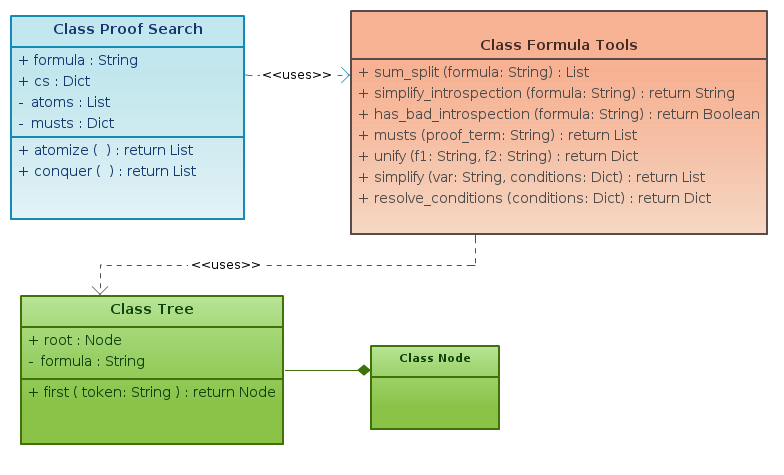
\includegraphics[width=1\textwidth]{Figures/uml_j-logic.png}
	\label{uml}
\end{figure}


\subsubsection[ProofSearch]{\texttt{ProofSearch}}
This class can be considered as the core logic of this project. It takes the user input, evaluates the justification formula and finally returns if the formula is provable or not. If it is, the output will also contain a proof.

\subsubsection[FormulaTools]{\texttt{FormulaTools}}
The name of the module reveals already its usage. This module doesn't quite deserve to be called a class since it does not describe any model but simply serves as a box of tools that perform functions which are not solely related with the model \texttt{Tree} and \texttt{Node} nor with \texttt{ProofSearch}. It is something like a go-in-between for those. Removing this module would result in a lot of static methods for both the \texttt{Tree} and the \texttt{ProofSearch} class and for many of them it would not be clear where they would fit best. 

Its core responsibility lies modifying and analysing formulas. In contrast to that the \texttt{Tree} is only concerned with the single formula that it describes and the \texttt{ProofSearch} does not actually handle formulas itself but only evaluates the result of an action on a formula given and decides how to proceed.


\section{Selected Methods}
In this section I want to show and explain some of the more important and thus usually more complicated methods that make up the heart of the algorithm. The source code of the methods presented here are excerpts only and occasional their in line comments where shortened in order to keep the snippets as short as possible and to avoid unnecessary repetition of information since the code comments are very similar to the description presented in this chapter. The aim of this section is to provide a insight of the source code without the need to read through all of the attached source code. 

\subsection[atomize]{\texttt{atomize, ProofSearch}}
The method \texttt{atomize} can be seen as the whole \emph{divide} step of the algorithm. I was tempted to name it so but I did not change it although it would have fitted very nicely with the corresponding method \texttt{conquer} which will be presented here as well. I felt that the name \emph{atomize} carries more meaning than \emph{divide} and after all \emph{divide} and \emph{conquer} is more a general approach and does not fit a hundred percent this algorithm.

The method is a straight forward implementation of the algorithm in chapter~\ref{chap:Algorithm.divide}. It splits the formula for each application found and then tries to simplify all subformulas that start with a introspection. Subformulas that are not resolvable~\footnote{Such would be formulas that start with a introspection but cannot be simplified or formulas that contain a introspection on the left side of a application.} are removed, leaving only those that we call \emph{atoms}.

\begin{figure}[H]
	\caption{Excerpt $atomize$ from $ProofSearch$.}
    \vspace{-10pt}
	\lstinputlisting[firstline=2, lastline=17]{Figures/code/atomize.py}
	\vspace{-10pt}
\end{figure}

\subsection[musts]{\texttt{musts, FormulaTools}}
The method \emph{musts} expects a given proof term to be atomized already as it only distinguishes between introspection and application operations.
The algorithm takes the formula apart from top to bottom, generating new, smaller terms for every operation it takes apart until the remaining proof term is only a proof constant. 

Since the resolution of a application operation introduces a new $X$ variable and the resolution of a introspection operation replaces an existing $X$ variable with a new one, the current $i$ for a new \emph{X-wild} $X_i$ is stored and increased in \texttt{v\_count}.

\begin{figure}[H]
	\caption{Excerpt $musts$ from $FormulaTools$}
    \vspace{-10pt}
	\lstinputlisting[firstline=2, lastline=20]{Figures/code/musts.py}
	\vspace{-10pt}
\end{figure}

If for example the current justification term is $((a\cdot (!b)):F)$, it will taken apart into the two subformulas $(a:(X_i\rightarrow F))$ and $((!b):(X_i))$. Further since from $!b:X_i$ it follows $\exists X_j \quad s.t. \quad !b:(b:X_j)$, all $X_i$ that occurred up to now must be replaced by $(b:X_j)$. These values are stored in \texttt{assignments} and eventually replaced.

In the end we will have only proof constants remaining.

\subsection[unify]{\texttt{unify, FormulaTools}}
I spend probably most of my implementing time on this method, or rather on many its predecessors. It used to be a lot longer and more complicated because it differentiated various cases if a formula would contain one or another kind of variable. In this final implementation X or Y variables are handled the same on this level.

The method \texttt{unify} takes two formulas~\footnote{It is assumed that the only occurring operations are $\rightarrow$ and $:$. It would be easy to extend the code at this point but from what I can expect as input this is not necessary here.} as input and compares them on the basis of their tree structure. If the roots of both trees are operations and matching, the children of both Nodes are pushed on a stack to be further compared later on. If one of the trees being compared consists only of a leaf that does not match the other node we either have found a contradiction or a \emph{condition}. In the first case \texttt{None} will be return the method is stopped. In the other case we find a node with a variable for one tree it will be formed into a \emph{condition} for that variable, where the variable is the key and whatever we find in the other tree at this place is the value.

All those conditions are stored as tuples in a set and are returned in form of a python dictionary, where all conditions for one variable can be accessed by the variable itself as key. At the current state conditions that apply to the same variable may contradict each other, but this method is responsible only for collecting conditions and not evaluating them. This will done by the method \texttt{simplify} and in a further extension also in the method \texttt{resolve\_conditions}.

\begin{figure}[H]
	\caption{Excerpt $unify$ from $FormulaTools$.}
	\vspace{-10pt}
	\lstinputlisting[firstline=2, lastline=25]{Figures/code/unify.py}
	\vspace{-10pt}
\end{figure}


\subsection[simplify]{\texttt{simplify, FormulaTools}}

The aim of this method is that after it has run there is only one condition term left for the variable\footnote{In the source code the combination of the variable and its single condition is referred to as \emph{the chosen one}.} it takes as input and this variable does not occur anywhere else except as key to its condition. For example, if we have $ [(A \rightarrow B), X_2, (Y_1 \rightarrow Y_2)]$ as conditions for the variable $X_1$ and $[(X_1)]$ as condition for $X_2$ after running the method we get $[(A \rightarrow B)]$ as the only condition for $X_1$, $[((A \rightarrow B), (Y_1 \rightarrow Y_2)]$ for $X_2$ and also $[(A)]$ for the new found variable $Y_1$ and $[(B)]$ for the new found variable $Y_2$. Thus we have eliminated all occurrences of the variable $X_1$ and as a consequence of this we found new variables that were not present before. 

Implementing this method proved harder than first expected since I didn't anticipated the role of the new found variables at first. The method \texttt{resolve\_conditions} handles the order in which this method is called on each variable. It simply pushes the new found variables on top of its stack to make sure they are given more priority. Because \texttt{resolve\_conditions} needs to know the new variables the method \texttt{simplify} makes changes to the condition set in place and instead of returning the conditions as it might be expected, it returns the list of newfound variables.

\begin{figure}[H]
	\caption{Excerpt $simplify$ from $FormulaTools$.}
	\vspace{-10pt}
	\lstinputlisting[firstline=13, lastline=39]{Figures/code/simplify.py}
	\vspace{-10pt}
\end{figure}


\subsection[conquer]{\texttt{conquer, ProofSearch}}
Although the method \texttt{conquer} is the one returning the final result, the actual work is done by the method \texttt{conquer\_one\_atom}. As the name suggests it checks the provability of one atom only. \texttt{conquer} then simply summarizes the result of each atom and give a readable output.

\texttt{conquer\_one\_atom} is structured in two main loops. In the first loop it collects all possible configurations for each of the \emph{musts} of the atom. If for any \emph{must} no valid configuration can be found the method will terminate because one unprovable \emph{must} makes the whole atom unprovable.

\begin{figure}[H]
	\caption{First excerpt $conquer\_one\_ atom$ from $FormulaTools$.}
	\vspace{-10pt}
	\lstinputlisting[firstline=3, lastline=19]{Figures/code/conquer.py}
	\vspace{-10pt}
\end{figure}

The second loop then tries to find an overall configuration that is compatible with at least one of the configurations per \emph{must}. If at some stage there is no entry left in \texttt{merged\_conditions}, it means that the conditions posed by the new encountered configuration of the musts are not compatible with the old ones and thus the atom is not provable.

\begin{figure}[H]
	\caption{Second excerpt $conquer\_one\_ atom$ from $FormulaTools$.}
	\vspace{-10pt}
	\lstinputlisting[firstline=23, lastline=41]{Figures/code/conquer.py}
	\vspace{-10pt}
\end{figure}

\bigskip


\section{Tests}
The simple unittests I have written for this algorithm have been most important to the success of it. They served me in two ways: First to check if my code would behave and actually do what I expected it to do and second when I suddenly stumbled across an example or a situation where I did not know what I would expect I would simple write a test for it and see what happens, thus helping me to understand it better.
It is also because of the tests that I have found so many mistakes, some minor others essential, making me recode bits and parts again and again at a stage when I had hoped to be done with the coding.

As can be seen when looking at the source code not all all methods are tested on a same quality level. Methods that I deemed simple usually have only one or two tests. An example for that is \texttt{summarize} from \texttt{ProofSearch}, this methods simply rearranges the elements of a dictionary and returns a nice readable output that summarized the content of the original input. In contrast to this methods like \texttt{conquer} or the \texttt{\_\_str\_\_} from \texttt{Tree} which basically tests if the parsing of the formula works correctly.

To name some numbers, there are currently\footnote{Even though the program is finished it is still possible that I add more tests to get rid of any doubts, so the numbers are not fix.} a total of 66 tests, almost half of which are related to \texttt{ProofSearch}. 